% Etica e procedure operative per il radioamatore – 4ª edizione
% Traduzione italiana non ufficiale. Licenza CC BY-SA 4.0.
% Compilare con XeLaTeX (due passaggi).
\documentclass[10pt,oneside,openany]{book}

% ---------- pagina (stesso formato dell'originale: 568.98 x 759 pt) ----------
\usepackage[paperwidth=568.98bp,paperheight=759bp,
  left=26mm,right=18mm,top=21mm,bottom=23mm,
  headheight=14pt,headsep=6mm,footskip=10mm,marginparwidth=20mm]{geometry}

% ---------- lingua e caratteri ----------
\usepackage{fontspec}
\XeTeXgenerateactualtext=1
\usepackage{polyglossia}
\setmainlanguage{italian}
\defaultfontfeatures{Ligatures=TeX}
\setmainfont{SourceSerifPro}[Path=fonts/,Extension=.otf,
  UprightFont=*-Regular,ItalicFont=*-It,BoldFont=*-Semibold,BoldItalicFont=*-SemiboldIt,
  Numbers=OldStyle]
\setsansfont{SourceSans3}[Path=fonts/,Extension=.otf,
  UprightFont=*-Regular,ItalicFont=*-It,BoldFont=*-Semibold,BoldItalicFont=*-SemiboldIt,
  FontFace={l}{n}{*-Light},FontFace={l}{it}{*-LightIt},FontFace={b}{n}{*-Bold}]
\setmonofont{DejaVu Sans Mono}[Scale=0.82]
\newfontfamily\eoplightfont{SourceSans3}[Path=fonts/,Extension=.otf,UprightFont=*-Light,BoldFont=*-Regular]
\newfontfamily\eopcoverfont{SourceSans3}[Path=fonts/,Extension=.otf,UprightFont=*-Light,BoldFont=*-Regular,WordSpace={1.9,1.4,1}]
\newfontfamily\eopsymfont{SourceSans3}[Path=fonts/,Extension=.otf,UprightFont=*-Regular]
\newfontfamily\eopliningserif{SourceSerifPro}[Path=fonts/,Extension=.otf,UprightFont=*-Regular,BoldFont=*-Semibold,Numbers=Lining]
\usepackage{newunicodechar}
\newunicodechar{◦}{{\eopsymfont ◦}}
\makeatletter
\renewcommand\normalsize{\@setfontsize\normalsize{9.6}{12.7}%
  \abovedisplayskip 8pt plus2pt minus4pt\abovedisplayshortskip 0pt plus2pt
  \belowdisplayshortskip 4pt plus2pt minus2pt\belowdisplayskip \abovedisplayskip}
\renewcommand\small{\@setfontsize\small{8.8}{11.4}}
\makeatother
\normalsize
\usepackage[protrusion=true]{microtype}
\emergencystretch=2.5em
\frenchspacing

% ---------- colori ----------
\usepackage[table]{xcolor}
\definecolor{eopblue}{HTML}{1B78B8}
\definecolor{eopteal}{HTML}{0097B2}
\definecolor{eopcream}{HTML}{FCE8A2}
\definecolor{eopink}{HTML}{222222}
\definecolor{eophead}{HTML}{DCEBF5}
\definecolor{eopzebra}{HTML}{F3F7FA}
\definecolor{eopnoteback}{HTML}{EEF6F8}
\definecolor{eopaccent}{HTML}{C0392B}
\definecolor{bp200}{HTML}{E3EEF7}
\definecolor{bp500}{HTML}{EAF4E6}
\definecolor{bp2700}{HTML}{FBF3DF}
\color{eopink}

% ---------- pacchetti ----------
\usepackage{graphicx}
\usepackage{longtable,array}
\setlength{\LTleft}{0pt}\setlength{\LTright}{0pt}
\setlength{\LTpre}{2pt}\setlength{\LTpost}{10pt}
\usepackage{tikz}
\usepackage{fancyhdr}
\usepackage{needspace}
\usepackage{multicol}
\usepackage{enumitem}
\usepackage{fancyvrb}
\usepackage[most]{tcolorbox}
\usepackage[hang,flushmargin]{footmisc}
\usepackage{dblfnote}
\DFNalwaysdouble
\usepackage{xurl}
\usepackage{etoolbox}
\usepackage{amsmath}
\usepackage[bookmarksnumbered=false,bookmarksopen=true,unicode]{hyperref}
\hypersetup{colorlinks=true,linkcolor=eopblue,urlcolor=eopblue,citecolor=eopblue,
  pdftitle={Etica e procedure operative per il radioamatore – Quarta edizione (traduzione italiana non ufficiale)},
  pdfauthor={Traduzione non ufficiale di: IARU Region 1, Ethics and Operating Procedures for the Radio Amateur, 4th ed.},
  pdfsubject={Traduzione italiana non ufficiale, per uso personale. CC BY-SA 4.0},
  pdfkeywords={IARU, radioamatore, etica, procedure operative, EOP},
  pdflang={it-IT}}
\urlstyle{same}
\usepackage{bookmark}

% ---------- spaziature ----------
\setlength{\parindent}{0pt}
\setlength{\parskip}{3.6pt plus 1.2pt minus 0.8pt}
\setlist{itemsep=2pt,parsep=0pt,topsep=3pt,leftmargin=1.4em}
\setlist[itemize,1]{label={\color{eopteal}\textbullet}}
\setlist[itemize,2]{label={\color{eopteal}–}}
\setlist[enumerate,1]{label=\arabic*,font=\eopliningserif\color{eopblue}}
\setlist[enumerate,2]{label=\arabic{enumi}.\arabic*,font=\eopliningserif\color{eopblue},leftmargin=2.2em}
\providecommand{\tightlist}{\setlength{\itemsep}{1pt}\setlength{\parskip}{0pt}}
\renewcommand{\footnotesize}{\fontsize{7.7}{9.6}\selectfont}
\setlength{\footnotemargin}{1.6em}
\renewcommand{\footnoterule}{\vspace*{2pt}{\color{eopblue!60}\hrule width 30mm height 0.4pt}\vspace*{4pt}}
\setlength{\skip\footins}{12pt plus 4pt}
\renewcommand{\thefootnote}{\arabic{footnote}}
\makeatletter
\renewcommand{\@makefnmark}{\hbox{\textsuperscript{\eopliningserif\color{eopblue}\@thefnmark}}}
\makeatother
\setcounter{secnumdepth}{-1}
\widowpenalty=3000 \clubpenalty=3000 \raggedbottom

% ---------- testatina e piede ----------
\newcommand{\eopchapmark}{}
\newcommand{\eopsecmark}{}
\pagestyle{fancy}
\fancyhf{}
\renewcommand{\headrulewidth}{0pt}
\fancyhead[L]{\footnotesize\color{eopblue}\textsc{iaru} © 2026 · 4.2.0 \textcolor{eopblue!60}{·} \textsc{traduzione italiana non ufficiale}}
\fancyhead[R]{\footnotesize\hyperlink{abbreviazioni}{Abbreviazioni} \textcolor{eopblue!60}{·} \hyperlink{indice}{Indice}}
\fancyfoot[L]{\sffamily\footnotesize\thepage}
\fancyfoot[R]{\parbox[t]{0.88\textwidth}{\raggedleft\sffamily\footnotesize\eopchapmark\ifdefempty{\eopsecmark}{}{ \textcolor{eopblue!70}{·} \eopsecmark}}}
\fancypagestyle{plain}{\fancyhf{}\fancyfoot[L]{\sffamily\footnotesize\thepage}}
\fancypagestyle{eopempty}{\fancyhf{}}

% ---------- titoli ----------
\newcommand{\eopsc}[1]{{\addfontfeatures{Letters=SmallCaps}#1}}
\newcommand{\eoplead}[1]{\textsc{#1}}
\newcommand{\eoplabel}[1]{\textsc{#1}}
\newcommand{\eopbar}[1]{$\overline{\mbox{#1}}$}
\newcommand{\eopfnsep}{\textsuperscript{,}}

\newcommand{\eopheadfont}{\sffamily\fontseries{l}\selectfont\addfontfeatures{Letters=SmallCaps}}

\newcommand{\eopfront}[2]{%
  \clearpage\eopfrontcont{#1}{#2}}
\newcommand{\eopfrontcont}[2]{%
  \par\needspace{6\baselineskip}\addvspace{14pt}%
  \hypertarget{#2}{}\phantomsection\addcontentsline{toc}{chapter}{#1}%
  \renewcommand{\eopchapmark}{#1}\renewcommand{\eopsecmark}{}%
  {\fontsize{17}{21}\selectfont\eopheadfont\color{eopblue}#1\par}\nopagebreak\vspace{8pt}}

\newcommand{\eoppart}[2]{%
  \clearpage
  \ifstrequal{#1}{A}{\pagenumbering{arabic}\setcounter{page}{1}}{}%
  \thispagestyle{plain}%
  \phantomsection\addcontentsline{toc}{part}{Parte #1: #2}%
  \renewcommand{\eopchapmark}{Parte #1}\renewcommand{\eopsecmark}{}%
  \null\vfill
  \begin{tikzpicture}[remember picture,overlay]
    \fill[eopteal] (current page.north west) rectangle ([yshift=-62mm]current page.north east);
    \node[anchor=north east,font=\fontsize{9}{11}\selectfont\sffamily\color{eopcream},text width=120mm,align=right]
      at ([xshift=-14mm,yshift=-14mm]current page.north east)
      {Etica e procedure operative per il radioamatore\\Quarta edizione · traduzione italiana non ufficiale};
  \end{tikzpicture}%
  {\raggedright\fontsize{30}{36}\selectfont\eopheadfont\color{eopblue}%
   Parte #1:\\[2pt]#2\par}
  \vspace{4mm}{\color{eopteal}\rule{30mm}{1.2pt}}
  \vfill\vfill\clearpage}

\newcommand{\eopchapter}[2]{%
  \par\needspace{0.16\textheight}\addvspace{20pt}%
  {\color{eopteal}\rule{\linewidth}{0.5pt}}\par\nopagebreak\vspace{4pt}%
  \phantomsection\addcontentsline{toc}{chapter}{\protect\numberline{#1}#2}%
  \renewcommand{\eopchapmark}{#2}\renewcommand{\eopsecmark}{}%
  {\raggedright\fontsize{17}{21}\selectfont\eopheadfont\color{eopblue}%
   \makebox[0pt][r]{\eoplightfont #1\hspace{9pt}}#2\par}%
  \nopagebreak\vspace{10pt}}

\newcommand{\eopsection}[2]{%
  \par\needspace{5\baselineskip}\addvspace{12pt}%
  \phantomsection\pdfbookmark[1]{#1 #2}{s#1}%
  \renewcommand{\eopsecmark}{#1 #2}%
  {\raggedright\fontsize{11.5}{14}\selectfont\eopheadfont\color{eopblue}%
   \makebox[0pt][r]{\eoplightfont #1\hspace{9pt}}#2\par}%
  \nopagebreak\vspace{3pt}}

\newcommand{\eopsubsection}[2]{%
  \par\needspace{4\baselineskip}\addvspace{9pt}%
  \phantomsection\pdfbookmark[2]{#1 #2}{s#1}%
  {\raggedright\fontsize{11}{13.5}\selectfont\color{eopblue}%
   \makebox[0pt][r]{\eopliningserif\small #1\hspace{9pt}}#2\par}%
  \nopagebreak\vspace{2pt}}

\newcommand{\eopsubsubsection}[2]{%
  \par\needspace{4\baselineskip}\addvspace{7pt}%
  \phantomsection\pdfbookmark[3]{#1 #2}{s#1}%
  {\raggedright\fontsize{10}{12.5}\selectfont\itshape\color{eopblue}%
   \makebox[0pt][r]{\upshape\eopliningserif\small #1\hspace{9pt}}#2\par}%
  \nopagebreak\vspace{1pt}}

% ---------- ambienti ----------
\newenvironment{eopwarn}{%
  \par\addvspace{3pt}%
  \everypar{\llap{\raisebox{-0.5pt}{\sffamily\bfseries\large\color{eopaccent}!}\hspace{9pt}}\everypar{}}%
  }{\par\addvspace{3pt}}

\newtcolorbox{eopqso}{breakable,enhanced,colback=eopzebra,colframe=eopzebra,
  borderline west={2pt}{0pt}{eopteal},arc=0pt,outer arc=0pt,
  left=8pt,right=6pt,top=4pt,bottom=4pt,before skip=6pt,after skip=8pt}
\fvset{fontsize=\small,baselinestretch=1.15}

\newtcolorbox{eopdialogbox}{breakable,enhanced,colback=eopzebra,colframe=eopzebra,
  borderline west={2pt}{0pt}{eopteal},arc=0pt,outer arc=0pt,
  left=8pt,right=6pt,top=5pt,bottom=5pt,before skip=6pt,after skip=8pt,
  fontupper=\small\sffamily}
\newenvironment{eopdialog}{\begin{eopdialogbox}\setlength{\parskip}{3pt}%
  \everypar{\hangindent=1.1em\hangafter=1}}{\end{eopdialogbox}}

\newtcolorbox{eopnotebox}{breakable,enhanced,colback=eopnoteback,colframe=eopnoteback,
  arc=1.5pt,left=8pt,right=8pt,top=5pt,bottom=5pt,before skip=6pt,after skip=8pt,
  fontupper=\small\sffamily}
\newenvironment{eopnote}{\begin{eopnotebox}\setlength{\parskip}{3pt}%
  \everypar{\hangindent=1.1em\hangafter=1}}{\end{eopnotebox}}

\newenvironment{eoptable}[1]{%
  \par\small\setlength{\tabcolsep}{4pt}\renewcommand{\arraystretch}{1.12}%
  \begin{longtable}{#1}}{\end{longtable}\par}
\newenvironment{eopsmalltable}[1]{%
  \small\setlength{\tabcolsep}{4pt}\renewcommand{\arraystretch}{1.12}%
  \begin{tabular}{#1}}{\end{tabular}}
\newcommand{\eopth}[1]{{\sffamily\bfseries\color{eopblue}#1}}
\newcommand{\eoptablecaption}[2]{%
  \par\needspace{7\baselineskip}\addvspace{6pt}%
  {\sffamily\small\color{eopblue}\textbf{Tabella #1:} #2\par}\nopagebreak\vspace{1pt}}

\usepackage{wrapfig}
% larghezza di ogni figura come frazione della giustezza
\expandafter\def\csname eopfw@5-i\endcsname{0.56}
\expandafter\def\csname eopfw@5-ii\endcsname{0.56}
\expandafter\def\csname eopfw@7-i\endcsname{0.50}
\expandafter\def\csname eopfw@7-ii\endcsname{0.50}
\expandafter\def\csname eopfs@5-i\endcsname{r}
\expandafter\def\csname eopfs@5-ii\endcsname{l}
\expandafter\def\csname eopfs@7-i\endcsname{r}
\expandafter\def\csname eopfs@7-ii\endcsname{r}
\setlength{\columnsep}{5mm}
\makeatletter
\newcommand{\eopfigure}[3]{%
  \par
  \edef\eop@side{\csname eopfs@#2\endcsname}%
  \expandafter\eop@wrap\expandafter{\eop@side}{\csname eopfw@#2\endcsname}{#1}{#2}{#3}}
\newsavebox{\eop@figbox}
\newcommand{\eop@wrap}[5]{%
  \sbox{\eop@figbox}{\begin{minipage}[t]{#2\textwidth}
    \centering\includegraphics[width=\linewidth]{#3}\par\vspace{3pt}
    {\footnotesize\setlength{\parskip}{0pt}\raggedright\textbf{\color{eopblue}Figura #4:} #5\par}
  \end{minipage}}%
  \needspace{\dimexpr\ht\eop@figbox+\dp\eop@figbox+3\baselineskip\relax}%
  \begin{wrapfigure}{#1}{#2\textwidth}
    \vspace{-8pt}\usebox{\eop@figbox}\vspace{-2pt}
  \end{wrapfigure}}
\makeatother
\renewcommand{\topfraction}{0.9}\renewcommand{\textfraction}{0.1}
\renewcommand{\floatpagefraction}{0.75}
\setlength{\textfloatsep}{14pt plus 4pt minus 2pt}
\setlength{\floatsep}{14pt plus 4pt minus 2pt}

\newenvironment{eopabbrlist}{\par\setlength{\columnsep}{14pt}\begin{multicols}{2}\fontsize{7}{7.95}\selectfont\setlength{\parskip}{0pt}\interlinepenalty=10000\raggedright}{\end{multicols}}
\newlength{\eopabbrsep}\setlength{\eopabbrsep}{2.5pt plus 1.5pt}
\newcommand{\eopabbr}[2]{\par\vspace{\eopabbrsep}\hangindent=3.9em\hangafter=1\noindent
  \makebox[3.9em][l]{\sffamily\bfseries\color{eopblue}#1}#2\par}

% ---------- indice ----------
\makeatletter
\renewcommand*{\l@part}[2]{%
  \addpenalty{-\@highpenalty}\vskip 9pt plus 1pt
  {\noindent\sffamily\bfseries\color{eopblue}\eopsc{#1}\nobreak\hfill\nobreak\eopliningserif#2\par}%
  \vskip 2pt}
\renewcommand*{\l@chapter}[2]{%
  \addpenalty{-\@highpenalty}\vskip 2.5pt
  {\leftskip 2.2em\parindent -2.2em\rightskip 2.5em plus 1fil\parfillskip -2.5em
   \def\numberline##1{\hb@xt@2.2em{\eopliningserif\color{eopblue}##1\hfil}}%
   \eopsc{#1}\nobreak\leaders\hbox{$\m@th\mkern 6mu\hbox{\color{eopblue!45}.}\mkern 6mu$}\hfill\nobreak
   \hb@xt@2.5em{\hss\eopliningserif #2}\par}}
\makeatother

\begin{document}
\frontmatter
\pagenumbering{roman}

% ================= COPERTINA =================
\thispagestyle{eopempty}
\begin{tikzpicture}[remember picture,overlay]
  \node[inner sep=0pt] at (current page.center)
    {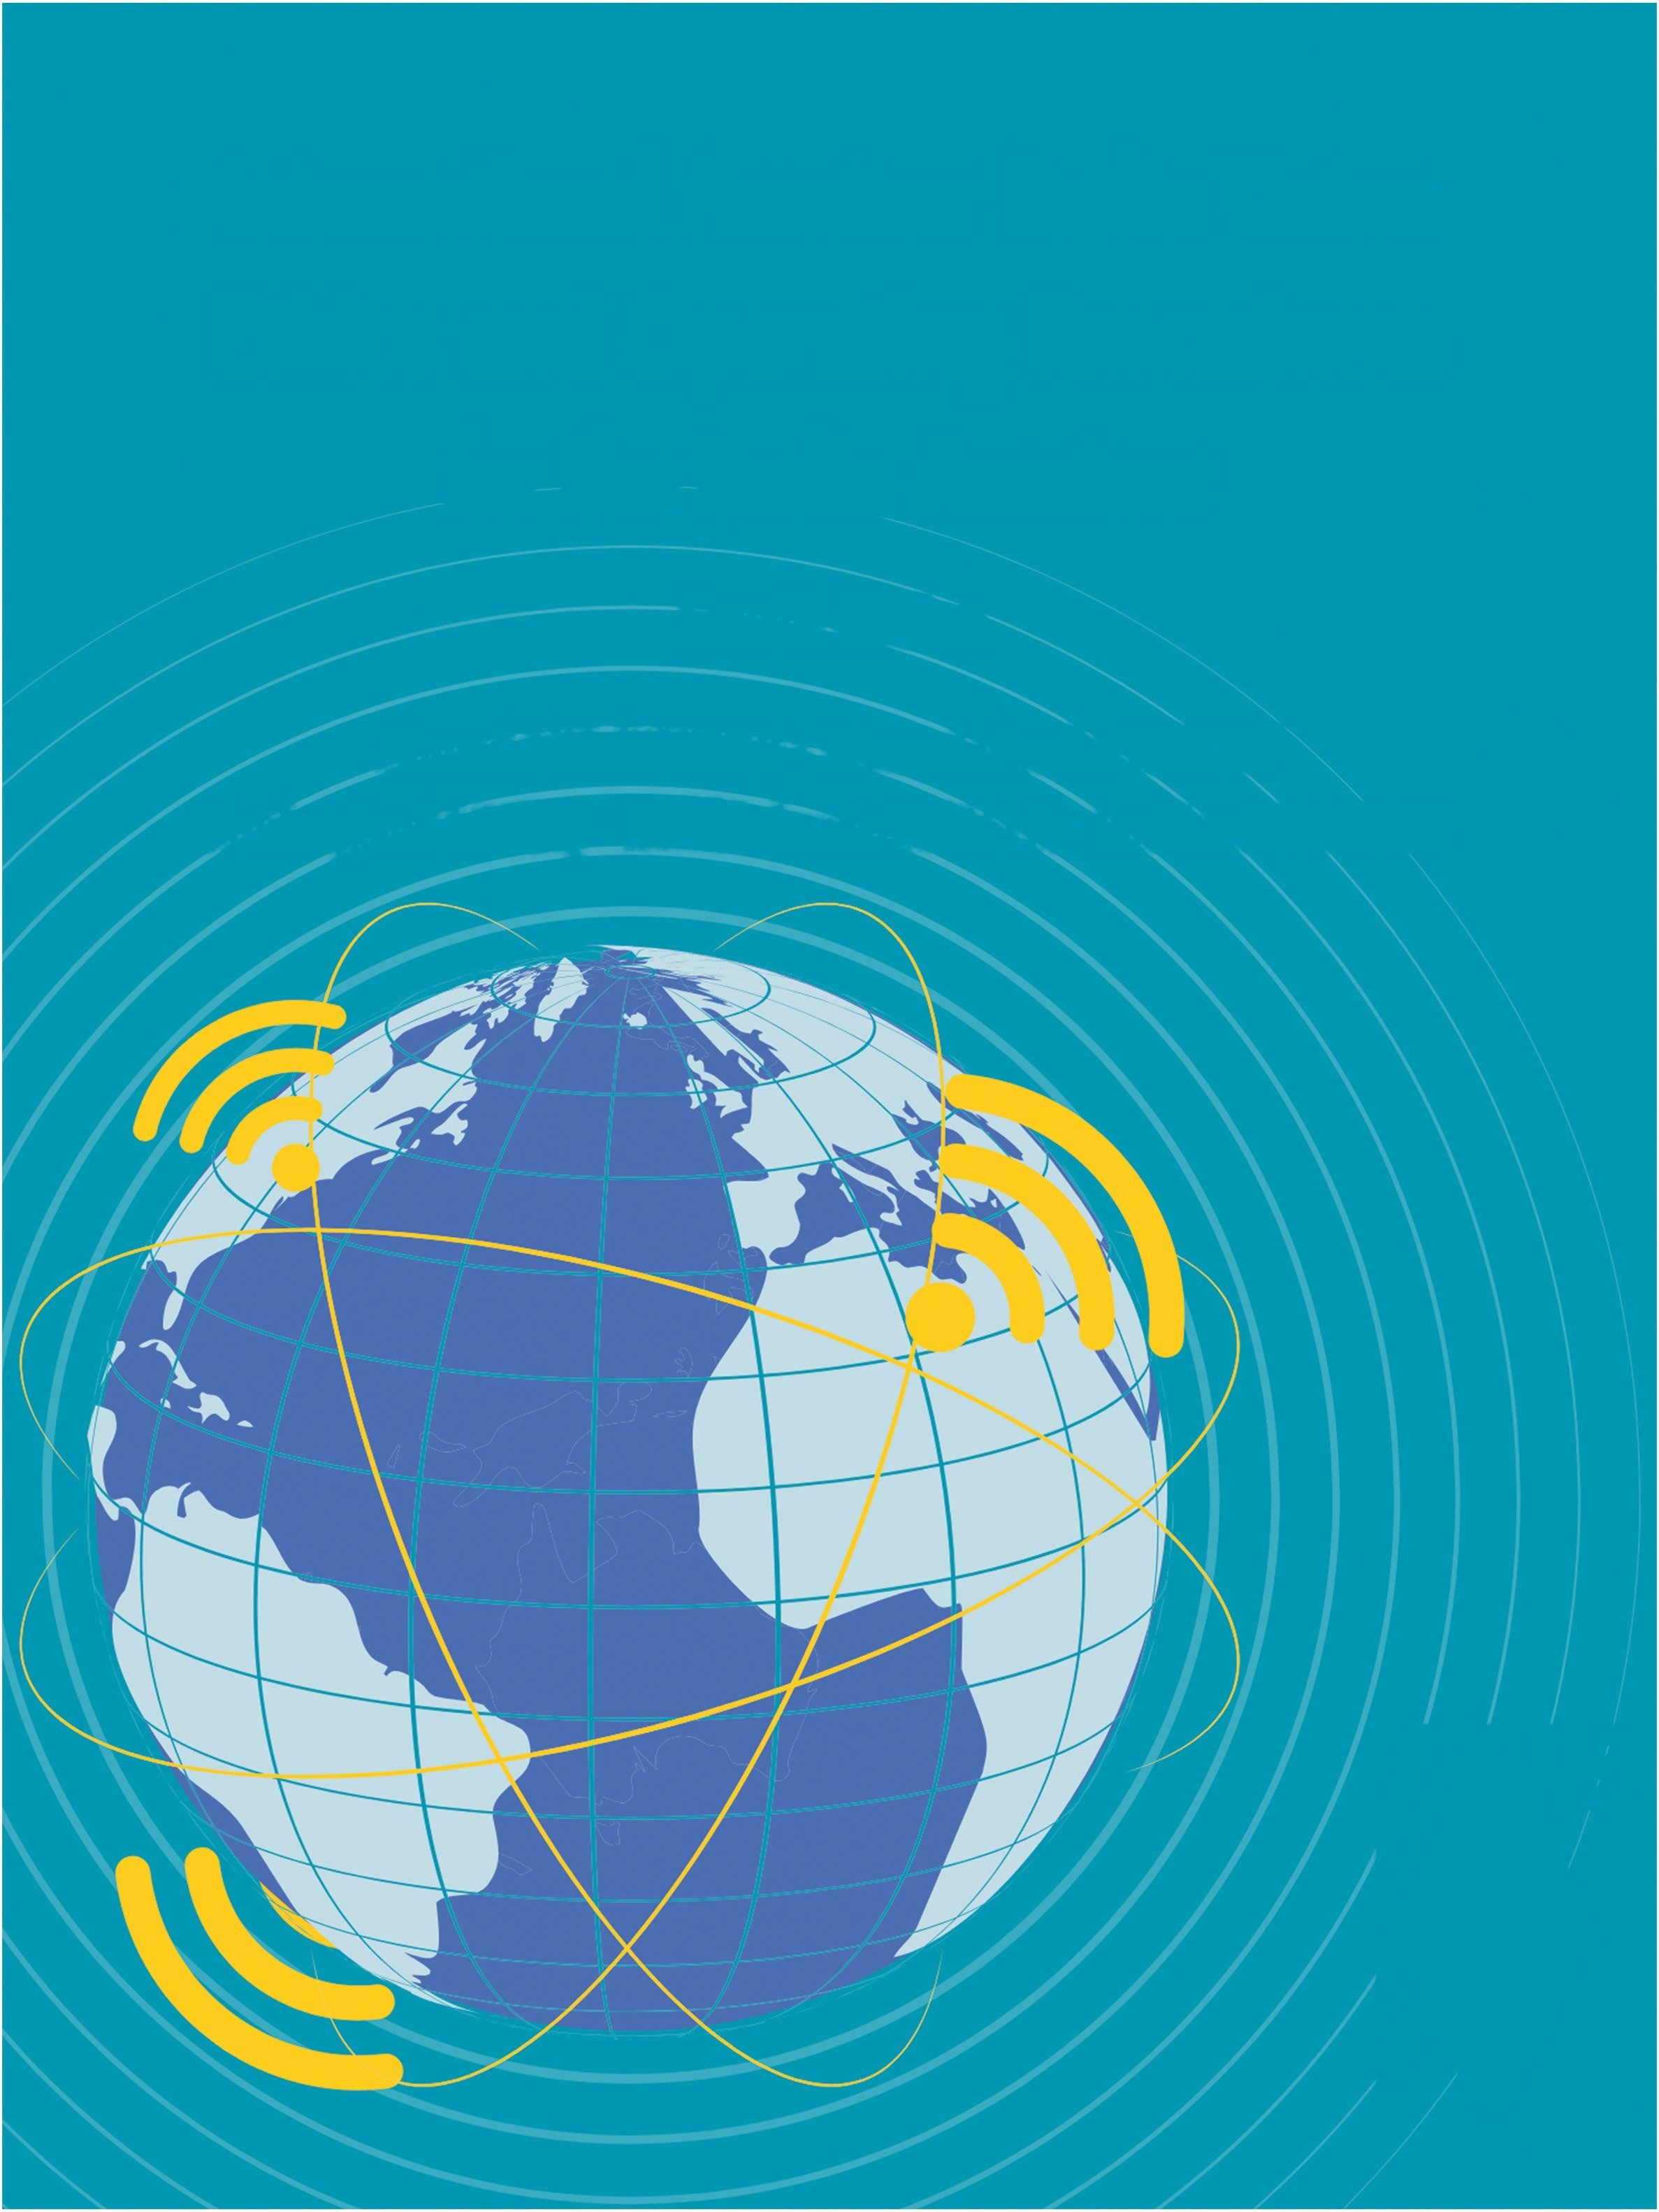
\includegraphics[width=\paperwidth,height=\paperheight]{img/cover-clean.jpg}};
  \node[anchor=north,text width=170mm,align=center,inner sep=0pt]
    at ([yshift=-20mm]current page.north)
    {\color{eopcream}\eopcoverfont\fontsize{28}{37}\selectfont
     International Amateur Radio Union\\
     Etica e procedure operative\\
     per il radioamatore\par
     \vspace{6mm}{\fontsize{16}{20}\selectfont Quarta edizione}\par
     \vspace{5mm}{\fontsize{12}{17}\selectfont
       Ahmad AlHoli 9K2DB · Marco Colombo IU2DXF\\
       Frode Igland LA6VQ · Rafal Lukawiecki EI6LA · Ian Suart GM4AUP}};
  \node[anchor=south east,draw=eopcream,line width=0.8pt,rounded corners=3pt,
        fill=eopteal!85!black,inner xsep=9pt,inner ysep=7pt,text width=40mm,align=center]
    at ([xshift=-10mm,yshift=12mm]current page.south east)
    {\color{eopcream}\sffamily\fontsize{8.5}{11}\selectfont
     \textbf{TRADUZIONE ITALIANA\\NON UFFICIALE}\\[2pt]
     per uso personale\\non approvata da IARU né da ARI};
\end{tikzpicture}
\null\clearpage

% ================= FRONTESPIZIO E DIRITTI (una sola pagina) =================
\thispagestyle{eopempty}
\vspace*{2mm}
{\raggedright\color{eopblue}\eopheadfont
 {\fontsize{12}{15}\selectfont International Amateur Radio Union\par}
 \vspace{5pt}
 {\fontsize{24}{29}\selectfont Etica e procedure operative\\per il radioamatore\par}
 \vspace{7pt}
 {\fontsize{13}{16}\selectfont Quarta edizione\par}}
\vspace{10mm}
\noindent\begin{minipage}[t]{0.48\linewidth}
{\sffamily\small\color{eopblue}\eopsc{autori}\par}\vspace{2pt}
Ahmad AlHoli 9K2DB\\Marco Colombo IU2DXF\\Frode Igland LA6VQ\\Ian Suart GM4AUP\par
\end{minipage}\hfill
\begin{minipage}[t]{0.48\linewidth}
{\sffamily\small\color{eopblue}\eopsc{autore e curatore}\par}\vspace{2pt}
Rafal Lukawiecki EI6LA\par
\end{minipage}\par
\vspace{10mm}
\begin{tcolorbox}[enhanced,colback=eopnoteback,colframe=eopteal,boxrule=0.6pt,arc=2pt,
  left=9pt,right=9pt,top=7pt,bottom=7pt,fontupper=\small]
{\sffamily\bfseries\color{eopblue}TRADUZIONE ITALIANA NON UFFICIALE – PER USO PERSONALE}\par\vspace{3pt}
Questa traduzione è stata realizzata a titolo personale, per studio e consultazione.
Non è una traduzione ufficiale dell'IARU e non è stata revisionata, approvata né certificata
dall'ARI – Associazione Radioamatori Italiani. In caso di differenze fa fede l'edizione originale
in lingua inglese, disponibile sul
\href{https://www.iaru-r1.org/on-the-air/eop/}{sito di IARU Region 1}.
\end{tcolorbox}
\vspace{3mm}
{\small Repository della traduzione:
\href{https://github.com/BBerry2020/iaru-eop-it}{\nolinkurl{github.com/BBerry2020/iaru-eop-it}}\par}
\vfill
{\color{eopteal}\rule{\linewidth}{0.4pt}}\par\vspace{6pt}
{\footnotesize\setlength{\parskip}{5pt}
\textbf{Edizione originale.} \emph{International Amateur Radio Union Ethics and Operating Procedures
for the Radio Amateur}, Fourth Edition, Revision 4.2.0. Copyright © 2026 International Amateur
Radio Union Region 1. Rilasciata con licenza Creative Commons Attribuzione – Condividi allo stesso
modo 4.0 Internazionale (CC BY-SA 4.0):
\href{https://creativecommons.org/licenses/by-sa/4.0/deed.it}{\nolinkurl{creativecommons.org/licenses/by-sa/4.0}}.
Pagina ufficiale dell'edizione originale:
\href{https://www.iaru-r1.org/on-the-air/eop/}{Codes of Conduct | International Amateur Radio Union (IARU)}.

Pubblicata da International Amateur Radio Union Region 1 (IARU R1), c/o Baer-Nutz-AG,
Scheuermattstrasse 8A, CH-6330 Cham ZG, Svizzera ·
\href{mailto:eop@iaru-r1.org}{eop@iaru-r1.org} · ISBN 978-3-9526620-0-7 (PDF eBook, inglese).
Questa traduzione non ha un ISBN proprio.

\textbf{Copertina.} Immagine di Silvano Ancelotti © 2025, usata secondo la licenza CC BY 4.0
(\href{https://creativecommons.org/licenses/by/4.0}{\nolinkurl{creativecommons.org/licenses/by/4.0}});
in questa edizione è stata modificata rimuovendo il testo originale e il logo IARU.

\textbf{Traduzione italiana.} Copyright © 2026 i contributori del repository
\href{https://github.com/BBerry2020/iaru-eop-it}{\nolinkurl{github.com/BBerry2020/iaru-eop-it}}.
Rilasciata anch'essa con licenza CC BY-SA 4.0, come richiesto dalla licenza dell'originale.
Il testo è tradotto in italiano senza modifiche di contenuto. Le note del traduttore sono segnalate
con [N.d.T.]. Le formule operative usate in aria (chiamate, esempi di QSO) sono lasciate nella forma
originale. Traduzione realizzata con l'ausilio di strumenti di intelligenza artificiale.

Bozza 0.1 · novembre 2026 · Composto in Source Serif e Source Sans.\par}
\clearpage

% ================= INDICE =================
\hypertarget{indice}{}
\renewcommand{\eopchapmark}{Indice}\renewcommand{\eopsecmark}{}
{\fontsize{17}{21}\selectfont\eopheadfont\color{eopblue}Indice\par}\vspace{10pt}
\phantomsection\addcontentsline{toc}{chapter}{Indice}
\makeatletter\@starttoc{toc}\makeatother
\clearpage

\input{body.tex}

% ================= QUARTA DI COPERTINA =================
\clearpage
\thispagestyle{eopempty}
\begin{tikzpicture}[remember picture,overlay]
  \fill[eopteal] (current page.south west) rectangle (current page.north east);
  \node[anchor=south west,text width=120mm,align=left,inner sep=0pt]
    at ([xshift=22mm,yshift=26mm]current page.south west)
    {\color{eopcream}\sffamily\fontsize{9}{12.5}\selectfont
     Traduzione italiana non ufficiale di \emph{Ethics and Operating Procedures for the
     Radio Amateur}, Fourth Edition, Revision 4.2.0 © 2026 International Amateur Radio
     Union Region 1. Licenza CC BY-SA 4.0.\\[4pt]
     Non approvata dall'IARU né certificata dall'ARI. In caso di differenze fa fede l'edizione inglese.\\[4pt]
     github.com/BBerry2020/iaru-eop-it};
\end{tikzpicture}
\null
\end{document}
